Для начала мы преобразуем изображение в черно-белое.

\begin{figure}[ht!]
    \centering
    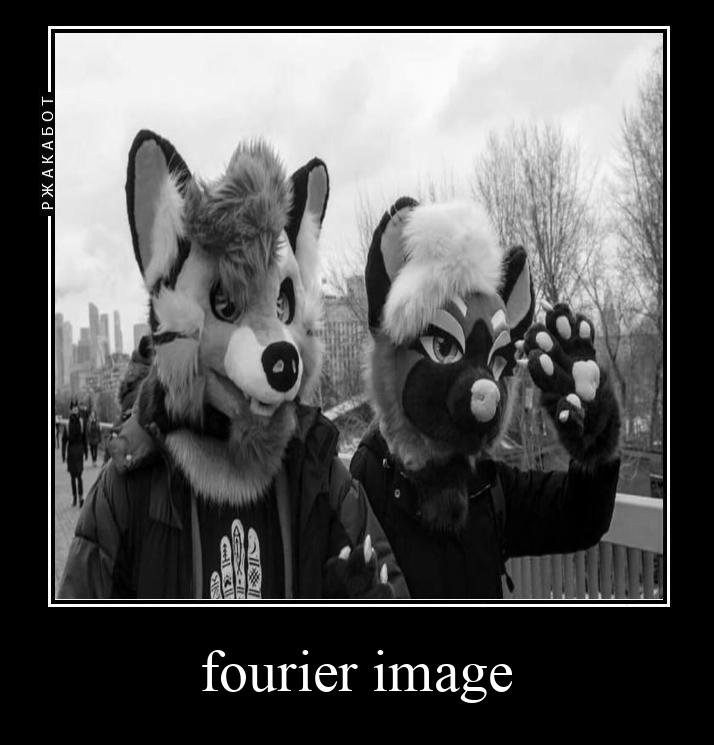
\includegraphics[width=0.5\textwidth]{/Users/nikolajprovorov/Yandex.Disk-368690@edu.itmo.ru.localized/Lab6_Furry_series/bw.png}
    \caption{Черно-белое изображение}
\end{figure}

Зададим матрицу ядра выделения краев:

\begin{equation}
    K = 
    \begin{bmatrix}
        -1 & -1 & -1 \\
        -1 & 8 & -1 \\
        -1 & -1 & -1
    \end{bmatrix}
\end{equation}

Найдем свертку исходного изображения с ядром и тд и тп, короче вот результат:

\clearpage

\begin{figure}[ht!]
    \centering
    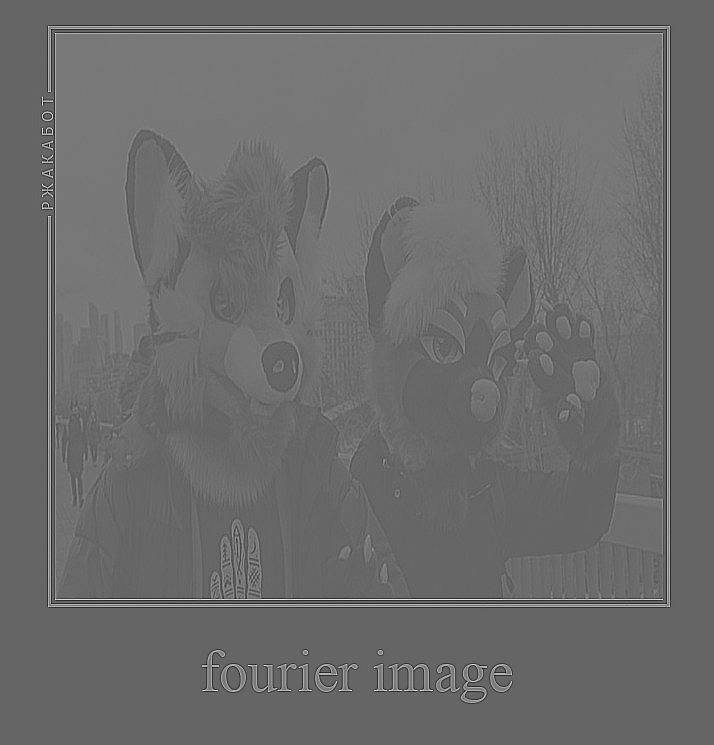
\includegraphics[width=0.5\textwidth]{/Users/nikolajprovorov/Yandex.Disk-368690@edu.itmo.ru.localized/Lab6_Furry_series/edge_x.png}
    \caption{Выделение краев изображения}
\end{figure}

Ну получилось очень даже неплохо, контрастность конечно пострадала, и сильно, но зато какие края!

Давайте посмотрим теперь на результат всего вот того фурье:

\begin{figure}[ht!]
    \centering
    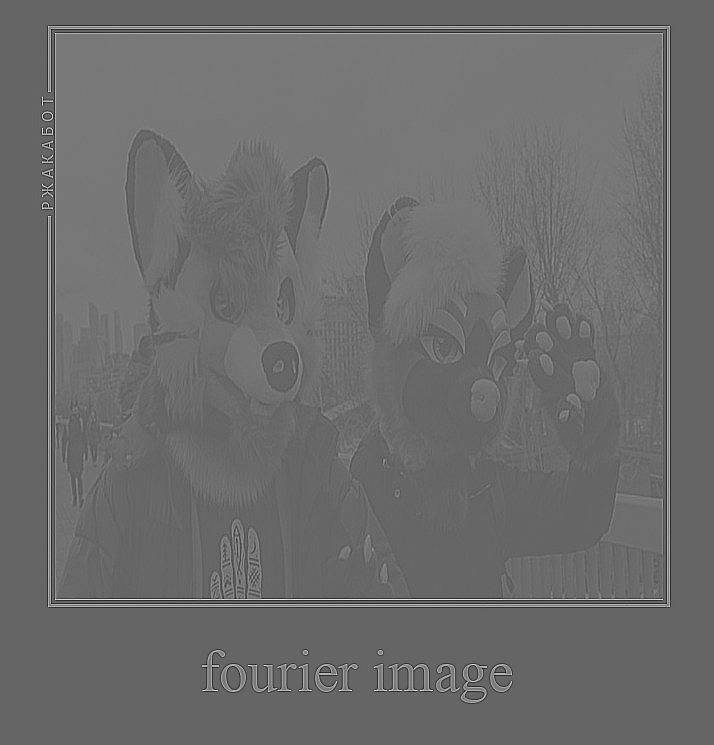
\includegraphics[width=0.5\textwidth]{/Users/nikolajprovorov/Yandex.Disk-368690@edu.itmo.ru.localized/Lab6_Furry_series/edge_x.png}
    \caption{Выделение краев изображения}
\end{figure}

О, прикол, совпали. Теорема о свертке работает корректно.